\documentclass[12pt,twocolumn]{article}
\usepackage{graphicx}
\usepackage{multicol}

\begin{document}

\begin{multicols}{2}
\title{Developing Disposable Wireless Sensor Networks}
\author{
    Zak Rubin  \\
    Computer Engineering \\
    UC Santa Cruz \\
    zrubin@soe.ucsc.edu \\
  \and
    H. Blake Skinner \\
    Computer Engineering \\
    UC Santa Cruz \\
    hskinner@soe.ucsc.edu
}
\maketitle
\end{multicols}

\begin{abstract}
Ad-hoc wireless sensor networks are predicted to increase in use significantly as advances in their core
hardware components continue.  They have already attracted considerable interest in academia and have
been successfully deployed for a variety of applications.  Despite advances in this area, cost and power
limitations remain the major obstacles to their use.

In this paper we explore the general problem of transferring data around a network
at minimal cost.  We present several protocols to transfer data across an ad-hoc network while
preserving the data's locality.  We will explore the problem of exchanging throughput for power
savings and will demonstrate what is possible in terms of through-put and power use with hardware
currently available on the market.  With this we hope to demonstrate the cost trade-offs associated
with wireless ad-hoc networks today how throughput can be sacrificed for power savings.

%Wireless sensor networks are predicted to increase in use significantly as advances in their core
%hardware components continue.  There are already many distributed, wireless sensor networks in use for
%a variety of applications, including wildlife conservation, security, and general purpose data-transfer
%networks.  Despite advances in the private sector and the research community in these areas, the
%primary limiting factor for such networks remain: cost and power consumption.
%
%In this paper, we would like to explore the general problem of transferring data around a network
%while preserving both the information and its locality.  Cost remains an issue in such network, as
%even a small cost is multiplied among many nodes.  Though memory has gotten increasingly cheap, there
%remain cut-offs between different models of chips, and even a few KBs of memory can make a significant
%difference in the project's budget.  We propose a several bare-bones protocols for synchronizing data,
%which can achieve reasonable through-put rates using a minimum of power and instruction memory.  We
%will demonstrate the through-put rates achievable with our system and relate them to cost, based on
%hardware currently available.
%
%In this paper we would like to explore low-power wireless sensor networks.  Sensor networks are predicted
%to increase in use significantly as advances in their core hardware components continue.  
%
%We have developed an extremely low-cost wireless sensor node, and have maximized its life by implementing a variety of power-conservation techniques. We introduce a localization system using received signal strength indicators provided when the wireless transceiver receives a packet to account for variations in measurements due to distance. We first demonstrate our system in  ContikiOS. Next we construct twenty of these nodes using off-the-shelf hardware on an extremely limited budget.  Finally, we also construct a gateway to enable communication between simulated nodes and hardware. 

{\bf Keywords:} sensor networks, low power
\end{abstract}


\section{Introduction}

Wireless sensor networks generally consist of a large number of small computers, or nodes, often built using micro-controllers.
There has been increasing interest in being able to construct such a network with and manage it with a fully distributed,
ad-hoc protocol.  This has been enabled by advances in the size, power consumption, and overall efficiency of the
core hardware components of the network, along with advances in development and simulation tools.  Sensor networks have
already generated a considerable amount of interest among academic researchers, numerous private companies including
start-ups, and with various government, especially military, organizations.

Monetary cost and power consumption continue to be limiting factors, however, and although the quality of hardware expected to
continue to improve,
applications involving wireless sensor networks often require, hundreds, or even thousands of nodes,
even small differences in cost are multiplied.
Furthermore, engineers designing these sensor networks must select between hardware components currently available on
the market, which can introduce considerable price-thresholds into the design process.  For example, the difference in cost
between a micro-controller with 8MB and 32MB of flash memory is only a few dollars, but this could easily represent a
thousands of dollars of cost difference between a network requiring less than 8MB of memory on each node and a network
requiring more than 8MB.  Furthermore, the power consumption of larger chips is greater as well, meaning a few extra
kilo-bytes of memory could also add battery and logistical costs.  Smaller micro-controllers also have less IO pins and
a generally have a slower clock-speed so thresholds exist in around those parameters as well.  Although the overall efficiency of
hardware is expected to improve while cost continues to decrease, wireless sensor engineers will have to contend with price/feature
thresholds for the foreseeable future.

In this paper, we would like to explore the cost of building a low power wireless network.  We propose several protocols
designed to minimize the total cost of a network, in terms of hardware and power usage.  We then demonstrate the throughput and
other network characteristics possible with these schemes, which are not ideal, but are workable for many applications, and
represents the minimum cost/functionality available with current technology.  We believe this serves as a useful demonstration
of what can be expected from a functional, bare-bones wireless sensor network and the cost and difficulty of implementing it.

The protocols we discuss could be implemented with minimal difficulty, from scratch, on even the lowest-end micro-controllers
available.  We also discuss implementing them on Contiki~\cite{contiki},
an open-source operating system for small-scale networked devices which is accompanied by an open-source simulator,
Cooja~\cite{cooja}.  With this we hope to demonstrate the capabilities and cost of a minimally-effective distributed
wireless sensor network and how it can be applied to a variety of applications.

%Wireless sensor nodes consist of low-cost microcontrollers with a few sensors attached. Their low cost, small size, and low power consumption make them extremely attractive for deployment over large areas or areas inaccessible to humans. However, this benefit precludes the ability to repair or maintain a specific individual node. As such, nodes need to be as cheap and power efficient as possible.
\section{Related Work}

\begin{quote}
\emph{``There’s Plenty of Room at the Bottom.''} – Richard Feynman
\end{quote}

Work on this was inspired after an investigation of Mainland’s paper that implemented a network that took actions based on an energy cost to reward ratio [1]. Primary criticisms included the cost of actual hardware and the relative inefficiency of the network communication. Additionally, we wanted to investigate what OS solutions existed besides TinyOS.

\subsection{Hardware}

\subsection{Network Communication}

\subsection{Sensor Network Operating Systems}

Mainland’s paper simulated the nodes in TinyOS. TinyOS [2]
Nano-RK is an operating system developed at Carnegie-Mellon University. RK stands for Resource Kernel, as it attempts to meet an energy budget by limiting CPU cycles or network usage [3]. 

There are a number of other microcontroller operating systems such as EMERALDS [4], but none could be found that would run on the limited resources of our microcontroller and still have wireless functionality.

ContikiOS [5]
\section{Design Considerations}
\label{section:design_considerations}

Cost remains a major limiting factor in the adoption of sensor networks.  Though the performance-to-price ratio of
hardware is expected to continue to improve, even small differences in price are multiplied across numerous nodes,
and the cookie-cutter manufacturing process of modern digital hardware, which has delivered increasingly powerful
chips for increasingly low costs, also presents cost thresholds to the design process.  This is not likely to change
anytime soon.

We present several protocols designed to create a minimal-effort, minimal-cost, low-power distributed sensor network
which can be implemented with relatively little effort without using external infrastructure, such as micro-kernel or
embedded OSs like EMERALD~\cite{zuberi99} or TinyOS~\cite{tinyos}.  We do this with low-end micro-controllers, such
as the ATtiny~\cite{attinyds}, in mind.

The primary mechanism to save power on a sensor network is to turn the node's radio off.  This presents an inherent
challenge, especially for peer-to-peer systems because when the radio is off, the node is effectively removed from
the network.  We explore two different strategies for tackling this problem, the first, discussed in
Section~\ref{section:heart_beat_protocol} is to dynamically put the nodes
on a synchronized schedule, the other, discussed in Section~\ref{section:random_dc} is to turn the radio on and off
based on random duty cycles.


\section{GumboNode}

\begin{figure}[h!]
  \centering
  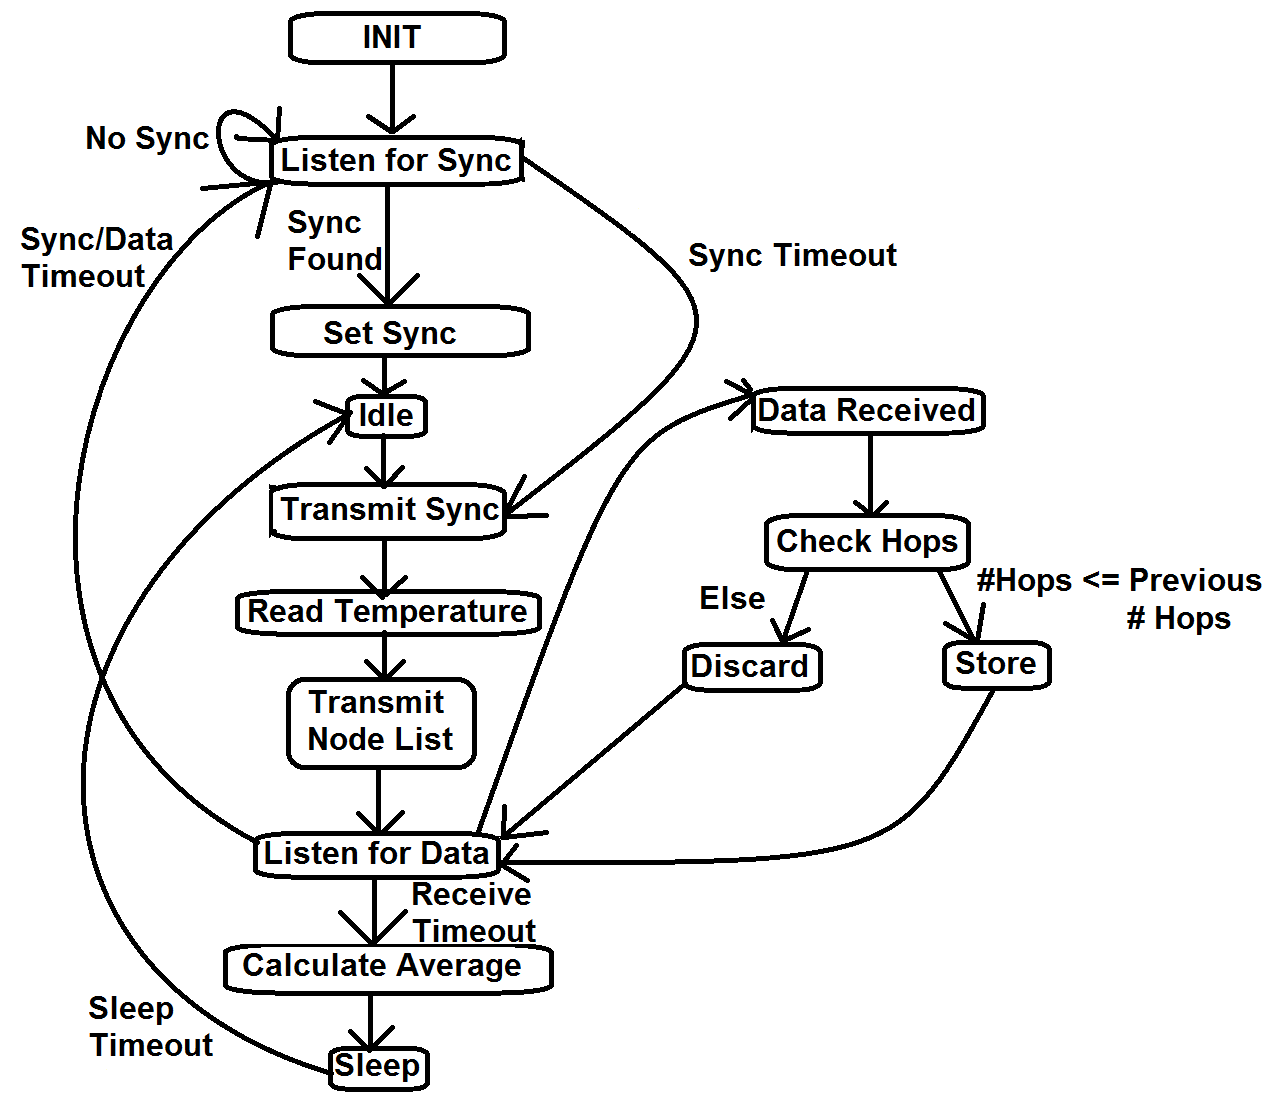
\includegraphics[width=0.5\textwidth]{images/algorithm_flowchart.png}
  \caption{A flowchart of the communication protocol.
  \label{img:flowchart}
  }
\end{figure}

\begin{figure}[h!]
  \centering
  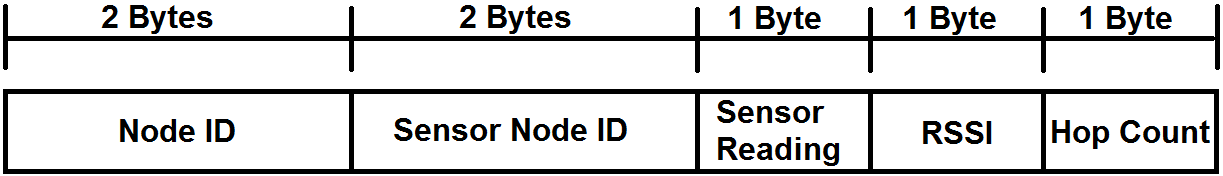
\includegraphics[width=0.5\textwidth]{images/packet_structure.png}
  \caption{Sensor packet list structure.
  \label{img:flowchart}
  }
\end{figure}

We developed GumboNodes. GumboNodes are barebones sensor nodes consisting of a microcontroller, a wireless transceiver, a sensor, and a battery. In our specific hardware, the system already comes on-board with a temperature sensor. 

We selected the ATTiny85 as the microcontroller for the chip. The ATTiny85 is a low-cost, low-power 8-bit processor. It is Arduino-compatible and has a wide range of options to optimize the processor for power consumption. Table 1 provides power information from the datasheet [6]. In the lowest power mode, the processor uses less than 2 μA. There are only two ways to wake the chip from this deep sleep: an external interrupt caused by a logic level change on an input pin, or periodically by an internal oscillator known as the watchdog timer. The watchdog timer has maximum time limit of 8 seconds after which the microcontroller automatically wakes up and enters idle state. The system may immediately be put back to sleep, or act after it wakes up a certain number of times.

The Texas Instruments CC2500 was selected as the wireless chip. The CC2500 is a low-level 2.4GHz wireless transceiver. Communication occurs over a 4-wire serial perhiperal interface (SPI) [7]. The ATTiny85 we selected lacks an onboard SPI interface, but has a universal serial interface (USI) that is capable of interfacing with the transceiver. The CC2500 also has a temperature sensor on-board, which served as our sensor. 

A flowchart of the node’s behavior is provided in Figure 1. After power-on, the system immediately goes into receive mode.
\section{Evaluation}
\label{section:evaluation}

%
% power consumption of the ATTiny85
%
\begin{table*}%[h!]
  \begin{center}
  
  \begin{tabular}{| c | c | c |}

  \hline
  \textbf{Mode} & \textbf{Typical Consumption} & \textbf{Max Consumption} \\
  \hline
  Active      & 5 mA & 8 mA \\
  Idle        & 1.2 mA & 2 mA \\
  Power-Down  & 2 $\mu$A & 2 $\mu$A \\
  \hline
  
  \end{tabular}
  \end{center}
  \caption{Power Consumption of ATTiny85 Modes at 8 MHz at 3V.
  \label{table:attiny85_power}  
  }
\end{table*}

%
% power consumption of the CC2500
%
\begin{table*}%[h!]
  \begin{center}
  
  \begin{tabular}{| c | c | c |}

  \hline
  \textbf{Mode} & \textbf{Minimum Consumption} & \textbf{Max Consumption} \\
  \hline
  Power-Down        & 400 nA & 160 $\mu$A \\
  Idle              & 1.2 mA & 2 mA \\
  Temperature-Read  & 1.5 mA & 1.5 mA \\
  TX Mode (2.4 Kbaud) & 11.1 mA & 21.5 mA \\
  RX Mode (2.4 Kbaud) & 14.5 mA & 17.0 mA \\
  \hline
  
  \end{tabular}  
  \end{center}
  \caption{Power Consumption of the CC2500 modes at 3V.
  \label{table:cc2500_power}  
  }
\end{table*}

%
% bill of materials
%
\begin{table*}%[h!]
  \begin{center}
  
  \begin{tabular}{| c | c | c | c |}

  \hline
  \textbf{Equipment} & \textbf{Cost at 1} & \textbf{Cost at 10} & \textbf{Cost at 100} \\
  \hline
  ATTiny85-20PU     & \$1.29 & \$1.08 & \$0.74 \\
  CC2500            & \$1.29 & \$1.08 & \$0.74 \\
  Battery (CR2450)  & \$1.29 & \$1.08 & \$0.74 \\
  Total             & \$1.29 & \$1.08 & \$0.74 \\
  \hline
  
  \end{tabular}  
  \end{center}
  \caption{Bill of Materials and Per-Part Cost on Different Scales of Production (as of November 2013).
  \label{table:bill}
  }
\end{table*}

%
% power consumption
%
\begin{table*}
  \begin{center}
  
  \begin{tabular}{| c | c | c |}

  \hline
  \textbf{Mode} & \textbf{Calculated} & \textbf{Measured} \\
  \hline
  Power-Down        & 2.4 $\mu$A & \\
  Idle              & & \\
  Temp Read         & & \\
  TX Read           & & \\
  RX Read           & & \\
  \hline
  
  \end{tabular}  
  \end{center}
  \caption{Power consumption.
  \label{table:power_consumption}
  }
\end{table*}

In this section we describe our investigation into sensor node communication. We built the nodes in software 

\subsection{Software Simulation}

Software simulation of the nodes was performed using Contiki OS. 

\subsection{Hardware}

As the primary purpose of this project is to produce inexpensive sensor networks, we built 20 nodes over a 2-week period. The total cost was \$158.60. After our hardware arrived we proceeded to run two experiments: one investigating power consumption, and one investigating large network tests.

\subsubsection{Hardware Costs}

Table 3 shows the overall parts cost. CC2500 and ATTiny costs were taken from Mouser.com. CR2450 cost information came from Amazon for cost at 1, and AliExpress for cost at 10 and 1000. Costs not included are PCB fabrication, as the system has not left the breadboard phase at the time of this writing. Also not included are shipping costs as the lightweight nature of the components (The heaviest component being the battery at 6.8 grams) meant that shipping was not a significant cost at any magnitude. The breadboard prototypes cost a total of \$7.59 per unit.

\subsubsection{Power Consumption}

We ran int

\subsection{Intercommunication}

\begin{figure}[h!]
  \centering
  
\includegraphics[width=0.5\textwidth]{images/textbook.png}
  \caption{Project cost measured in textbooks.
  \label{img:flowchart}
  }
\end{figure}

\begin{figure}[h!]
  \centering
  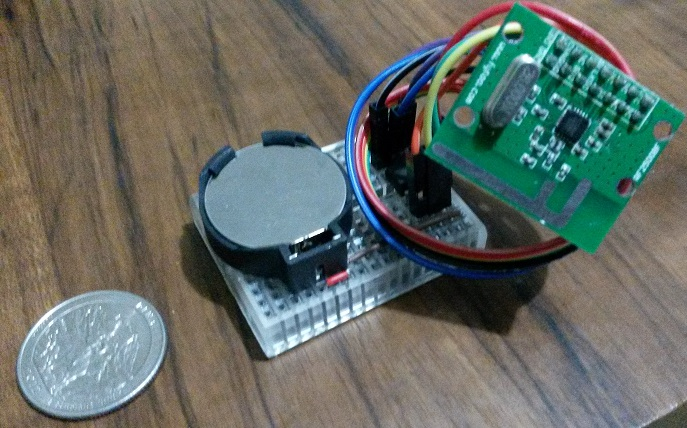
\includegraphics[width=0.5\textwidth]{images/phone_picture.png}
  \caption{Node on a breadboard.
  \label{img:flowchart}
  }
\end{figure}

While 20 nodes are fine for hardware simulation, we wanted to investigate a more realistic number of sensor nodes. However, it is not possible to install ContikiOS onto the microcontroller due to memory limitations. To enable communication in between the hardware and the software simulation we added an ATMega128RFA1. This microcontroller has a built-in Zigbee-compatible transceiver and is capable of running ContikiOS natively.

\section{Challenges}
\label{section:challenges}

The ATTiny85 is extremely limited on General Purpose Input Output (GPIO) pins. The entire chip only has 8 pins; after reset, power, and ground the user is left with only five pins to work with. 1
There are concerns of networks splitting and forming two separately synced networks, even more so in hardware where the watchdog is an imprecise timer. 

It was surprising how easily bad data . Werner-Allen et al. mention similar problems in their flooding time syncronization protocol. 

Ensuring a transmission is guaranteed to be received by at least 1 node was surprisingly difficult in smaller networks. The larger network test showed no sync loss, but on the 2-3 node network tests nodes fell out of sync around once per minute.

Lengths of cables caused problems in this low power environment. The jumper wires between the nodes and the transceiver were made by the lowest bidder, and had a tendency to lose parts of the signal. While not difficult to measure, we are confident that this significantly contributed to the packet errors. Along with this, the USB cable used for serial communication was too long, resulting in more frequent serial print errors until the Uno locked up and had to be reset. During the long-term network test the Uno would begin sending corrupted messages within an hour, and would lock up within four hours.
\section{Future Work}
\label{section:future_work}

Due to the short time period given on this project, the greatest limiting factor was time. The system merits much deeper investigation, and there is plenty to explore.

Despite multiple forms of error checking, bad data still arrived and propagated through the network quite quickly. LQI this does lend itself to interesting potential applications. RSSI and LQI numbers are subject to interference from Wi-Fi router, cell phones, microwaves, and other sources of 2.4 GHz interference.

The system's sleep current consumption was significantly higher than planned. Though the wake/sleep duty cycle chosen was not significantly impacted by our limitations. As the duty cycle decreases and the system spends more time in sleep, the need to achieve the proposed power consumption are more critical. With a 1 second wakeup every 10 minutes the system lasts a little over 9 days with our current power consumption, but over 2 years if had the system hit the ideal consumption numbers.
\section{Acknowledgements}

Our thanks to ACM SIGCHI for allowing us to modify templates they had developed.

\bibliographystyle{plain}
\bibliography{gumbo_bib}

\end{document}
